% !TEX encoding = IsoLatin                     
%cette premiÃère ligne permet au compilateur (souvent, dÃépend du compilateur) \LaTeX de reconnaitre l'encodage de votre fichier. 
%\documentclass[12pt,titlepage,twoside]{book}       %pour un livre
%\documentclass{report}
\documentclass[a3, 10pt,twoside]{article}          %pour un article
%\documentclass[twocolumn,amsfonts,showpacs,superscriptaddress,nofootinbib,aps,nolongbibliography]{revtex4-2}
%\documentclass[onecolumn,amsfonts,showpacs,superscriptaddress]{revtex4-1}

\usepackage{array,multirow,graphicx}
\usepackage[T1]{fontenc}  % For correct {}s in \texttt
\usepackage{accents}
\usepackage[francais]{babel}
\usepackage{amssymb, amssymb, amsthm}
\usepackage[utf8]{inputenc}             
\usepackage{amstext, amsfonts, a4}
\usepackage{pgf,pgfarrows,pgfautomata,pgfheaps,pgfnodes,pgfshade}
\usepackage[left=0.05cm,right=0.05cm,top=0.05cm,bottom=0.05cm,nohead]{geometry}
\usepackage{natbib}
%\usepackage{amsmath,amssymb}
\usepackage[pdfborder={0 0 0}]{hyperref}
\usepackage{xxcolor}
\usepackage{amscd}
\usepackage{dsfont}
\usepackage{float} 
\usepackage[Glenn]{fncychap} % Rejne Glenn\chapter
%\usetikzlibrary{circuits.ee.IEC}
\usepackage{lipsum} % pour générer du texte aléatoire

%\usepackage[tikz]{bclogo}
\usepackage{mathrsfs}%lagrangien
\usepackage{stmaryrd} %\llbracket
\usepackage{bbold}%Matrice 11
\usepackage{shapepar}
\usepackage{cancel}
\usepackage{bm}
\usepackage{pdfpages}
\usepackage[utf8]{inputenc}
\usepackage{marvosym}
\usepackage{enumitem}
\usepackage{import} % Charger le package import
\usepackage{listings} % Pour afficher du code MATLAB
\usepackage{pgfplots}
\usetikzlibrary {datavisualization}
\usetikzlibrary {arrows.meta,bending,positioning}
\usetikzlibrary {datavisualization.formats.functions}

\usepackage{tikz}
\usepackage[europeanresistor]{circuitikz}
\usepgflibrary {shadings}
%\usetikzlibrary{calc}
\usetikzlibrary{hobby, decorations.markings, arrows.meta}
\usetikzlibrary{decorations.markings} 
\usetikzlibrary{calc,intersections,through,backgrounds}
\usetikzlibrary {arrows.meta}


%%%%%%%%%%%%%%%%%%%%%%%%%%%%%%%%% Pour le tag
%\usepackage[utf8]{inputenc}
%\usepackage{fourier}
\usepackage{mathtools}
%\usepackage{cleveref}
\usepackage{xcolor}
%%%%%%%%%%%%%%%%%%%%%%%%%%%%%%%%%%


%%%%%%%%%%%%%%%%%%%%%%%%%%%%%%%%%%
\newcommand{\operatorvec}[1]{\hat{{\bm{#1}}}} % pour les operateur
\newcommand{\operator}[1]{\hat{\bm{#1}}} % pour les operaeur vecteur 
\newcommand{\operatortilde}[1]{\tilde{\bm{#1}}} % pour les opetateur avec un tilde
\newcommand{\operatortildevec}[1]{\tilde{\bm{#1}}}% pour les opetateur avec un tilde et vecteur 
%%%%%%%%%%%%%%%%%%%%%%%%%%%%%%%%%%

%\usepackage{tzplot}

%\usepakage{pstriks}
\usepackage[utf8]{inputenc}

%PREAMBULE pour schÃéma
\usepackage{pgfplots}
\usepackage{tikz}
%\usepackage[european resistor, european voltage, european current]{circuitikz}
%\usetikzlibrary{arrows,shapes,positioning}
%\usetikzlibrary{decorations.markings,decorations.pathmorphing,decorations.pathreplacing}
%\usetikzlibrary{calc,patterns,shapes.geometric}
\usetikzlibrary{patterns} % Pour les motifs comme les lignes diagonales
\usepackage{float} % Pour le placement 'H'
%FIN PREAMBULE

% PREAMBULE pour vercteur derivÃé
\usepackage[b]{esvect}    % For \vv

%\usepackage{caption}
%\usepackage{subcaption}

%\usepackage{graphicx}

\usepackage{fullpage}
\usepackage{eso-pic}
\usepackage{enumitem}

%\usepackage{pgfplots}
%\pgfplotsset{compat=1.17}



% --- Macro \xvec
\makeatletter
\newlength\xvec@height%
\newlength\xvec@depth%
\newlength\xvec@width%
\newcommand{\xvec}[2][]{%
  \ifmmode%
    \settoheight{\xvec@height}{$#2$}%
    \settodepth{\xvec@depth}{$#2$}%
    \settowidth{\xvec@width}{$#2$}%
  \else%
    \settoheight{\xvec@height}{#2}%
    \settodepth{\xvec@depth}{#2}%
    \settowidth{\xvec@width}{#2}%
  \fi%
  \def\xvec@arg{#1}%
  \def\xvec@dd{:}%
  \def\xvec@d{.}%
  \raisebox{.2ex}{\raisebox{\xvec@height}{\rlap{%
    \kern.05em%  (Because left edge of drawing is at .05em)
    \begin{tikzpicture}[scale=1]
    \pgfsetroundcap
    \draw (.05em,0)--(\xvec@width-.05em,0);
    \draw (\xvec@width-.05em,0)--(\xvec@width-.15em, .075em);
    \draw (\xvec@width-.05em,0)--(\xvec@width-.15em,-.075em);
    \ifx\xvec@arg\xvec@d%
      \fill(\xvec@width*.45,.5ex) circle (.5pt);%
    \else\ifx\xvec@arg\xvec@dd%
      \fill(\xvec@width*.30,.5ex) circle (.5pt);%
      \fill(\xvec@width*.65,.5ex) circle (.5pt);%
    \fi\fi%
    \end{tikzpicture}%
  }}}%
  #2%
}
\makeatother

% --- Override \vec with an invocation of \xvec.
\let\stdvec\vec
\renewcommand{\vec}[1]{\xvec[]{#1}}
% --- Define \dvec and \ddvec for dotted and double-dotted vectors.
\newcommand{\dvec}[1]{\xvec[.]{#1}}
\newcommand{\ddvec}[1]{\xvec[:]{#1}}
% FIN PREAMBULE


\def\pgf{\textsc{pgf}}
\def\pstricks{\textsc{pstricks}}
\def\Class#1{\hbox{\small#1}}
\def\bs{$\backslash$}

\def\Environment#1{\par\bigskip\noindent\textbf{Environment \texttt{#1}}\par}
\def\Command#1{\par\bigskip\noindent\textbf{Command \texttt{#1}}\par}
\long\def\Parameters#1{\medskip\noindent Parameters:
  \begin{enumerate}\itemsep=0pt\parskip=0pt
    #1
  \end{enumerate}}
\long\def\Description#1{\unskip\medskip\noindent Description: #1}
\def\Example{\par\medskip\noindent Example: }


\renewcommand*\descriptionlabel[1]{\hspace\labelsep\normalfont #1}


\def\declare#1{{\color{red!75!black}#1}}

\def\command#1{\list{}{\leftmargin=2em\itemindent-\leftmargin\def\makelabel##1{\hss##1}}%
\item\extractcommand#1@\par\topsep=0pt}
\def\endcommand{\endlist}
\def\extractcommand#1#2@{\strut\declare{\texttt{\string#1}}#2}


\def\environment#1{\list{}{\leftmargin=2em\itemindent-\leftmargin\def\makelabel##1{\hss##1}}%
\extractenvironement#1@\par\topsep=0pt}
\def\endenvironment{\endlist}
\def\extractenvironement#1#2@{%
\item{{\ttfamily\char`\\begin\char`\{\declare{#1}\char`\}}#2}%
  {\itemsep=0pt\parskip=0pt\item{\meta{environment contents}}%
  \item{\ttfamily\char`\\end\char`\{\declare{#1}\char`\}}}}


\def\smallpackage{\vbox\bgroup\package}
\def\endsmallpackage{\egroup\endpackage}
\def\package#1{\list{}{\leftmargin=2em\itemindent-\leftmargin\def\makelabel##1{\hss##1}}%
\extracttheme#1@\par\topsep=0pt}
\def\endpackage{\endlist}
\def\extracttheme#1#2@{%
\item{{{\ttfamily\char`\\usepackage}#2{\ttfamily\char`\{\declare{#1}\char`\}}}}}



\def\Environment#1{\par\bigskip\noindent\textbf{Environment \texttt{#1}}\par}
\def\Command#1{\par\bigskip\noindent\textbf{Command \texttt{#1}}\par}
\long\def\Parameters#1{\medskip\noindent Parameters:
  \begin{enumerate}\itemsep=0pt\parskip=0pt
    #1
  \end{enumerate}}
\long\def\Description#1{\unskip\medskip\noindent Description: #1}
\def\Example{\par\medskip\noindent Example: }

\newcommand{\w}[1]{\bf{#1}}\newcommand{\ww}[1]{\bf{#1}}
%\newcommand{\w}[1]{\vec{#1}}\newcommand{\ww}[1]{\overrightarrow{#1}}



\newcommand{\vertiii}[1]{{\left\vert\kern-0.25ex\left\vert\kern-0.25ex\left\vert#1\right\vert\kern-0.25ex\right\vert\kern-0.25ex\right\vert}}

%%%%%%%%%%%%%%%%%%%%%%%%%%%%%%%%%%%%%%%%%%%%%%%%%%%%%%%%%%%
    %%%%%%%% Accent Math
%%%%%%%%%%%%%%%%%%%%%%%%%%%%%%%%%%%%%%%%%%%%%%%%%%%%%%%%%%%
\makeatletter
\newcommand*{\math@auxii}[2][3]{{}\mkern#1mu\overline{\mkern-#1mu#2}}
\newcommand*{\math@auxi}[3][3]{\overset{\mkern#1mu\text{\scalebox{0.7}{#3}}\mkern-#1mu}{\smash{\math@auxii[#1]{#2}}\vphantom{#2}}}
\newcommand*{\mathco}[2][3]{\math@auxi[#1]{#2}{$\circ$}}
\newcommand*{\mathabc}[2][3]{\math@auxi[#1]{#2}{abc}}
\makeatother

%%%%%%%%%%%%%%%%%%%%%%%%%%%%%%%%%%%%%%%%%%%%%%%%%%%%%%%%%
%%%%algorithmes / pseudo code%%%
%%%%%%%%%%%%%%%%%%%%%%%%%%%%%%%%%%%%%%%%%%%%%%%%%%%%%%%%%%
\usepackage[french,ruled]{algorithm2e}

%%%%%
\usepackage{color,transparent}
%%%%%
%\usepackage{graphics,graphicx,subfigure,caption}
%\usepackage{graphics,graphicx,caption}
\usepackage{caption}
\usepackage{subcaption}
\usepackage{comment}
\usepackage{float} 
\setcounter{MaxMatrixCols}{30}%

%%%%%%%%%%%%%%%%%%%%%%%%%%%%%%%%%%%%%%%%
%%%%        Dimensions du texte (à adapter selon votre goût/le goût de l'Ãéditeur)
%%%%%%%%%%%%%%%%%%%%%%%%%%%%%%%%%%%%%%%%

\setlength\textwidth{19cm}          % largeur du texte
\setlength\topmargin{-1cm}          % marge en haut
\setlength\evensidemargin{-1cm}     % marge de gauche
\setlength\textheight{24cm}         % hauteur du texte
\setlength\oddsidemargin{\evensidemargin}

%%%%%%%%%%%%%%%%%%%%%%%%%%%%%%%%%%%%%%%%
%         D\'ecoupage des mots           %
%%%%%%%%%%%%%%%%%%%%%%%%%%%%%%%%%%%%%%%%
\hyphenation{}

%%%%%%%%%%%%%%%%%%%%%%%%%%%%%%%%%%%%%%%%
%%%%  Th\'eor\`emes, d\'efinitions, etc.
%%%%%%%%%%%%%%%%%%%%%%%%%%%%%%%%%%%%%%%%


% Il y a diffÃérents types d'ÃénoncÃés qui mÃéritent un environnement spÃécifique, voici une liste assez exhaustive. 
\theoremstyle{plain}
	\newtheorem{Theo}{Th\'eor\`eme}[section] %compteur commençant par le numÃéro de la section (on pourrait aussi faire commencer par le numÃéro de la sous-section - remplacer "section" par "subsection")
	\newtheorem{Prop}[Theo]{Proposition}        %mÃême compteur que pour les thÃéorÃèmes      
	\newtheorem{Prob}[Theo]{Probl\`eme}	    %idem
	\newtheorem{Lemm}[Theo]{Lemme}            %etc...
	\newtheorem{Coro}[Theo]{Corollaire}
	\newtheorem{Propr}[Theo]{Propri\'et\'e}
	\newtheorem{Conj}[Theo]{ Conjecture}
	\newtheorem{Aff}[Theo]{Affirmation}

    \newtheorem{TheoPrinc}{Th\'eor\`eme}     %compteur spÃécifique pour les thÃéorÃèmes les plus importants du papier
        
\theoremstyle{definition}
	\newtheorem{Defi}[Theo]{D\'efinition}
    \newtheorem{Exem}[Theo]{Exemple}
	\newtheorem{Nota}[Theo]{\Large Notation}

\theoremstyle{remark}
	\newtheorem{Rema}[Theo]{Remarque}
	\newtheorem{NB}[Theo]{N.B.}
	\newtheorem{Comm}[Theo]{Commentaire}
	\newtheorem{question}[Theo]{$\ast$ Question}
	\newtheorem{exer}[Theo]{Exercice}
	\newtheorem{Consequence}[Theo]{Conséquence}
	\newtheorem{Rap}[Theo]{Rappel}
	\newtheorem*{Merci}{Remerciements}
	
\usepackage{mdframed}

\mdfdefinestyle{propstyle}{%
linecolor=black,linewidth=2pt,%
hidealllines=true,
frametitlerule=true,%
frametitlebackgroundcolor=gray!20,
backgroundcolor=gray!10!white,
roundcorner=5pt,
innertopmargin=\topskip,
}

%\mdtheorem[style=propstyle]{prop}{Property}[chapter]
\mdtheorem[style=propstyle]{lemma}[prop]{Lemma}
\mdtheorem[style=propstyle]{TheoPrinc}{Th\'eor\`eme}[chapter]

% Définition d'un style personnalisé pour les Affirmations
\mdfdefinestyle{affirmestyle}{%
    linecolor=gray, % Couleur de la bordure
    linewidth=1pt, % Épaisseur de la bordure
    backgroundcolor=gray!10, % Couleur de fond (gris clair)
    roundcorner=5pt, % Coins arrondis
    innertopmargin=\topskip, % Marge intérieure
    skipabove=10pt, % Espace au-dessus du cadre
    skipbelow=10pt % Espace en-dessous du cadre
}

% Définition de l'environnement Affirmation
\theoremstyle{definition} % Style de théorème pour les affirmations
\newmdtheoremenv[style=affirmestyle]{aff}{Affirmation} % Environnement Affirmation avec le style personnalisé


	

%%%%%%%%%%%%%%%%%%%%%%%%%%%%%%%%%%%%%%%%
%%%%  Accolades, guillemets, etc.
%%%%%%%%%%%%%%%%%%%%%%%%%%%%%%%%%%%%%%%%

\def\ogg~{{\rm \og}}   % guillemets ouvrants
\def\fgg{{\rm \fg}}  % guillemets fermants



\def\nl{\newline}
\def\nn{\noindent}

\def\q{\nn}
\def\qq{\nn\quad}
\def\qqq{\nn\quad\quad}
\def\qqqq{\nn\quad\quad\quad}
\def\ce{\centerline}

%%%%%%%%%%%%%%%%%%%%%%%%%%%%%%%%%%%%%%%%
%%%%  Lettres et symboles math\'ematiques
%%%%%%%%%%%%%%%%%%%%%%%%%%%%%%%%%%%%%%%%

\def\emptyset{\varnothing}

%%%% Raccourcis pour les caractÃères gras mathÃématiques (ensembles R, N, Z, C etc)

\def\NN{{\mathbb N}}    %naturels
\def\ZZ{{\mathbb Z}}     %entiers relatifs
\def\RR{{\mathbb R}}    %rÃéels
\def\QQ{{\mathbb Q}}    %rÃéels
\def\CC{{\mathbb C}}    %complexes
\def\HH{{\mathbb H}}    %quaternions / espace hyperbolique
\def\AA{{\mathbb P}}     %espace projectif
\def\KK{{\mathbb K}}     %corps quelconques

\def\EE{{\mathbb E}}     %Experance
\def\VV{{\mathbb V}}     %Variance

%%%%%%raccourcis lettres calligraphiÃées
\def\cA{{\mathcal A}}  \def\cG{{\mathcal G}} \def\cM{{\mathcal M}} \def\cS{{\mathcal S}} \def\cB{{\mathcal B}}  \def\cH{{\mathcal H}} \def\cN{{\mathcal N}} \def\cT{{\mathcal T}} \def\cC{{\mathcal C}}  \def\cI{{\mathcal I}} \def\cO{{\mathcal O}} \def\cU{{\mathcal U}} \def\cD{{\mathcal D}}  \def\cJ{{\mathcal J}} \def\cP{{\mathcal P}} \def\cV{{\mathcal V}} \def\cE{{\mathcal E}}  \def\cK{{\mathcal K}} \def\cQ{{\mathcal Q}} \def\cW{{\mathcal W}} \def\cF{{\mathcal F}}  \def\cL{{\mathcal L}} \def\cR{{\mathcal R}} \def\cX{{\mathcal X}} \def\cY{{\mathcal Y}}  \def\cZ{{\mathcal Z}}

%%%%%%raccourcis lettres gothiques

\def\mfA{{\mathfrak A}} \def\mfA{{\mathfrak P}} \def\mfS{{\mathfrak S}}\def\mfZ{{\mathfrak Z}} \def\mfM{{\mathfrak M}} \def\mfQ{{\mathfrak Q}} \def\mfE{{\mathfrak E}} \def\mfL{{\mathfrak L}} \def\mfW{{\mathfrak W}} \def\mfR{{\mathfrak R}} \def\mfK{{\mathfrak K}} \def\mfX{{\mathfrak X}} \def\mfT{{\mathfrak T}} \def\mfJ{{\mathfrak J}} \def\mfC{{\mathfrak C}} \def\mfY{{\mathfrak Y}} \def\mfH{{\mathfrak H}} \def\mfV{{\mathfrak V}}\def\mfU{{\mathfrak U}}\def\mfG{{\mathfrak G}} \def\mfB{{\mathfrak B}} \def\mfI{{\mathfrak I}} \def\mfF{{\mathfrak F}} \def\mfN{{\mathfrak N}} \def\mfO{{\mathfrak O}} \def\mfD{{\mathfrak D}} 

\def\mfa{{\mathfrak a}} \def\mfp{{\mathfrak p}} \def\mfs{{\mathfrak s}}  \def\mfz{{\mathfrak z}} \def\mfm{{\mathfrak m}} \def\mfq{{\mathfrak q}}  \def\mfe{{\mathfrak e}} \def\mfl{{\mathfrak l}} \def\mfw{{\mathfrak w}} \def\mfr{{\mathfrak r}} \def\mfk{{\mathfrak k}} \def\mfx{{\mathfrak x}} \def\mft{{\mathfrak t}} \def\mfj{{\mathfrak j}} \def\mfc{{\mathfrak c}} \def\mfy{{\mathfrak y}} \def\mfh{{\mathfrak h}} \def\mfv{{\mathfrak v}} \def\mfu{{\mathfrak u}} \def\mfg{{\mathfrak g}} \def\mfb{{\mathfrak b}} \def\mfi{{\mathfrak i}} \def\mff{{\mathfrak f}} \def\mfn{{\mathfrak n}} \def\mfo{{\mathfrak o}} \def\mfd{{\mathfrak d}} 



%%raccourcis texte
\newcommand{\nbh}{\nobreakdash-\hspace*{0pt}}	% trait d'union insÃécable
\newcommand{\cad}{c'est\nbh \`a\nbh dire}		% c.-??-d.
\newcommand{\Cad}{C'est\nbh \`a\nbh dire}		% C.-??-d.

%%opÃérateurs   (ajoutez les raccourcis que vous voulez pour les opÃérateurs dont avez besoin)
\newcommand{\pgcd}{\operatorname{pgcd}}
\newcommand{\ppcm}{\operatorname{ppcm}}
\newcommand{\GL}{\operatorname{GL}}             %groupe linÃéaire
\newcommand{\Sp}{\mathsf{Sp}}			    %spectre
\newcommand{\End}{\operatorname{End}}         %Endomorphismes
\newcommand\Aut{\operatorname{Aut}}		  %etc...
\newcommand\ct{\operatorname{cotan}}         %cotangente
\newcommand{\dx}{\partial_x}                    
\newcommand{\dy}{\partial_y}
\newcommand{\Ker}{\operatorname{Ker}}
\newcommand{\Id}{\operatorname{Id}}
%\def\Im{\operatorname{Im}}                            %dans ce cas, \newcommand ne va pas marcher car la commande \Im existe dÃéjà. On utilise alors  \def de tex.

%%%%% a ajouter 

\usepackage{xcolor}
\newcommand{\varitem}[3][black]{%
  \item[%
   \colorbox{#2}{\textcolor{#1}{\makebox(5.5,7){#3}}}%
  ]
}


%%%%

\usepackage{scalerel}
\usepackage{xcolor}
\usepackage{stackengine}
\usepgflibrary {shadings}


\usetikzlibrary {decorations.pathmorphing}

\newcommand\dangersign[1]{%
    \renewcommand\stacktype{L}%
    \scaleto{\stackon[1.3pt]{\color{red}$\triangle$}{\tiny !}}{#1}%
}

\usepackage{tikz}
\tikzset{every picture/.style={execute at begin picture={\shorthandoff{:;!?};}}}
\tikzstyle{every picture}+=[remember picture]
\tikzstyle{na} = [shape=rectangle,inner sep=0pt]

% Commandes pour les flèches textuelles
\newcommand{\ptFleche}[2]{		% Déclaration d'une extrémité de flèche
    \tikz[baseline=(#1.base)]\node[na](#1){#2};
  }
%\newcommand{\Fleche}[5][thick]{	% Dessin de la flèche
%    \begin{tikzpicture}[overlay]
%        \path[->,#1](#2) edge [out=#4, in=#5] (#3);
%    \end{tikzpicture}
%  }
  
% \newcommand{\Flecheprim}[5][thick]{	% Dessin de la flèche
%    \begin{tikzpicture}[overlay]
%        \path[->,#1](#2) edge [out=#4, in=#5] (#3);
%    \end{tikzpicture}
%  }
%
\usepackage{marvosym}
\usepackage{changepage}
 


\begin{document}
	\section{Les données } 
	\begin{itemize}
		\item[date :] 2024-04-24
		\item[scanes :] 89-97-102-108
		\item[Parametres :] With1 , DeadtimeDMD, With1$\_$bis, DeadtimeDMD$\_$bis
	\end{itemize}
	
	\begin{figure}[ht]
        \centering
        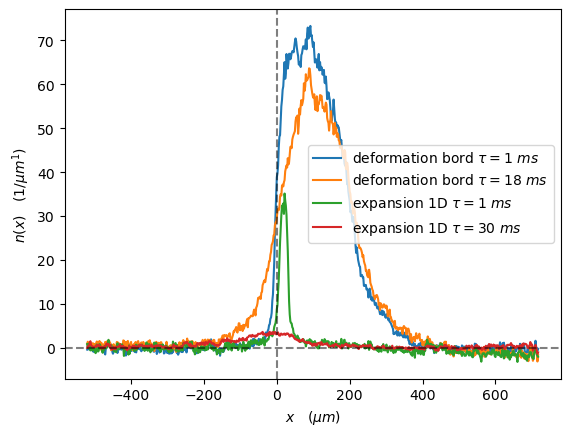
\includegraphics[width=0.5\textwidth]{figures/donnees_24-04-2024}
        \caption{les profiles du 24-04-2024 : 
         }
        \label{fig:donnes}
    \end{figure}
    
    \begin{enumerate}[label =\alph*)]
    	\item "deformation bord $\tau = 1~ ms$ (\ref{fig:donnes}) : profile longitudinale des données $1 ~ms$ aprés la selection en $x = 0$ 
    	\item "deformation bord $\tau = 18~ ms$ (\ref{fig:donnes}): profile longitudinale des données après $18~ms$  de déformation du bord
    	\item "expansion 1D $\tau =1~ms$"(\ref{fig:donnes}) : profile longitudinale des données après $1~ms$ d'expansion.
    	\item "expansion 1D $\tau =30~ms$" (\ref{fig:donnes}): profile longitudinale des données après $30~ms$ d'expansion.	
    \end{enumerate}

	{~}\\
	
	\begin{enumerate}[label =\Alph*)]

		\item Système semi-infinie pour $x\geq 0$ :
			\begin{enumerate}[label =\alph*)]
				\item Système dans une potentiel quartique  :
					\begin{itemize}[label =$\bullet$]
						\item fréquence transverse : $\omega_\perp \overset{exp}{=} 2 \pi * 2.56 ~KHz$	
						\item la densité spatial théorique : $n_0 = n_p $  sur les données "deformation bord $\tau = 1~ ms$" (\ref{fig:donnes}), je mesure   $n_p \overset{exp}{=} 56.6 ~{\mu m}^{-1}$.
					\end{itemize}
				\item Selection de $x\geq 0$  :
					\begin{itemize}[label =$\bullet$]
						%\item[$\circ$] le graphe ("deformation bord $\tau = 1~ ms$ (\ref{fig:donnes})) représente le profile longitudinale des données $1 ~ms$ aprés la selection en $x = 0$ 
						\item la densité spatial théorique : $n_0 = n_p \Theta (x) $  
						\item garde le potentiel transverse
					\end{itemize}
			\end{enumerate}
			
			 
		\item Deformation du bord : 
			\begin{itemize}[label =$\bullet$]
				\item[$\circ$] "deformation bord $\tau = 1~ ms$ (\ref{fig:donnes}) : le profile longitudinale des données apres $1~ms$ de déformation du bord
				\item[$\circ$] "deformation bord $\tau = 18~ ms$ (\ref{fig:donnes}) : le profile longitudinale des données apres $18~ms$ de déformation du bord
				\item garde le potentiel transverse %$\omega_\perp \overset{exp}{=} 2 \pi * 2.56 ~KHz$
				\item temps de déformation du bord $\tau = 18~ ms$	
			\end{itemize}
		\item Mesure locale de distribution de rapidité , Expansion 1D   : 
			\begin{enumerate}[label =\alph*)]
				\item Local : selection de la tranche $[ x_0 - \ell/2 , x_0 + \ell/2 ]$:
					\begin{itemize}[label =$\bullet$]
						\item $x_0 = 19.6 ~\mu m $ (trouvé avec un ajustement gaussien sur "expansion 1D $\tau =1~ms$" (\ref{fig:donnes}) ) 
						\item $\ell = 24.78 ~ \mu m $ (trouvé en faisant la différence des positions des extremums du gradient de s données "expansion 1D $\tau =1~ms$" (\ref{fig:donnes}) ) 	
					\end{itemize}
				\item Expansion :
					\begin{itemize}[label =$\bullet$]
						\item[$\circ$] "expansion 1D $\tau =1~ms$" : profile longitudinale des données après $1~ms$ d'expansion.
						\item[$\circ$] "expansion 1D $\tau =30~ms$" : profile longitudinale des données après $30~ms$ d'expansion.
						\item temps de déformation du bord $\tau = 18~ ms$		
					\end{itemize}
				\item[$\bullet$] garde le potentiel transverse %$\omega_\perp \overset{exp}{=} 2 \pi * 2.56 ~KHz$


			\end{enumerate}
			

	\end{enumerate}
	
	\section{Simulation GHD}
		\begin{figure}[ht]
			\begin{subfigure}[b]{0.45\textwidth}
        		\centering
        		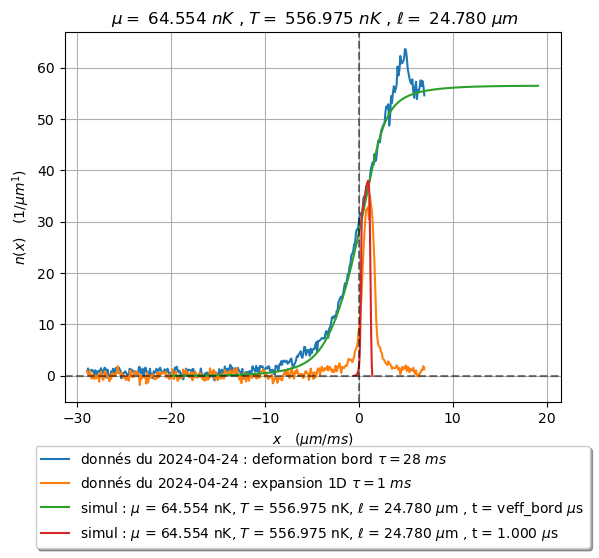
\includegraphics[width=\textwidth]{figures/simul_deformation_18_24-04-2024}
        		\caption{les profiles du 24-04-2024}
        		\label{fig:sub1}
    		\end{subfigure}
    		\vspace{1em}

    		\begin{subfigure}[b]{0.45\textwidth}
        		\centering
        		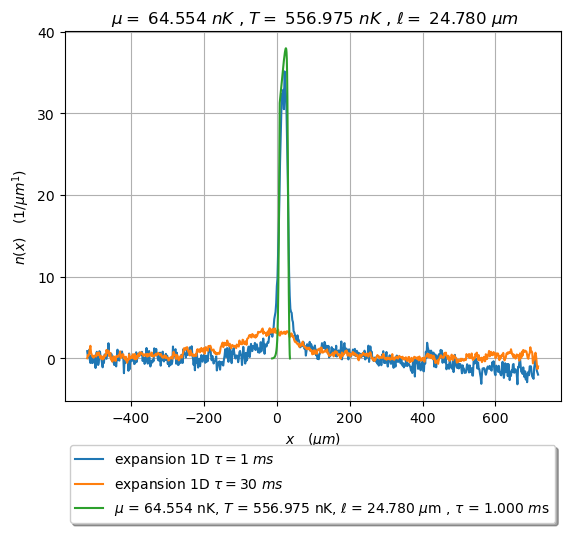
\includegraphics[width=\textwidth]{figures/simul_expansion_1_24-04-2024}
        		\caption{expension : $\tau = 1ms$}
        		\label{fig:sub1}
    		\end{subfigure}
    		\hfill
     		\begin{subfigure}[b]{0.45\textwidth}
        		\centering
        		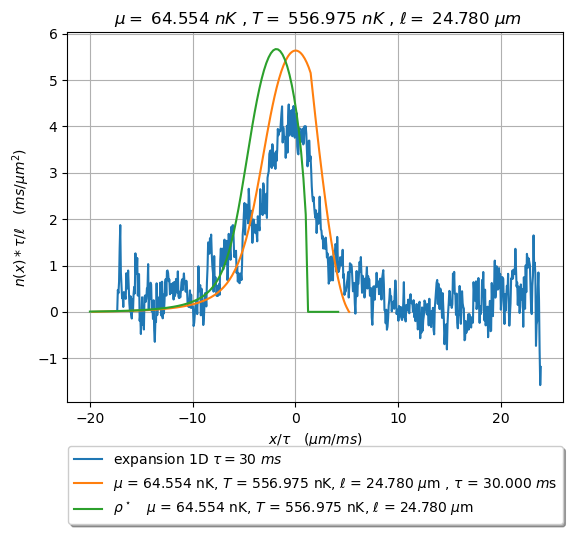
\includegraphics[width=\textwidth]{figures/simul_expansion_30_24-04-2024}
        		\caption{expension : $\tau = 30ms$}
        		\label{fig:sub1}
    		\end{subfigure}
				
		\end{figure}

	
		\subsection{Méthode 1 : } 
		
			\begin{enumerate}[label =\Alph*)]
				\item On extrais la temperature $T$ en faisant un ajustement sur le profil de bord 	
			\end{enumerate}

			


	
	
	
	
	\begin{figure}[ht]
    \centering
    % Première sous-figure
    \begin{subfigure}[b]{0.45\textwidth}
        \centering
        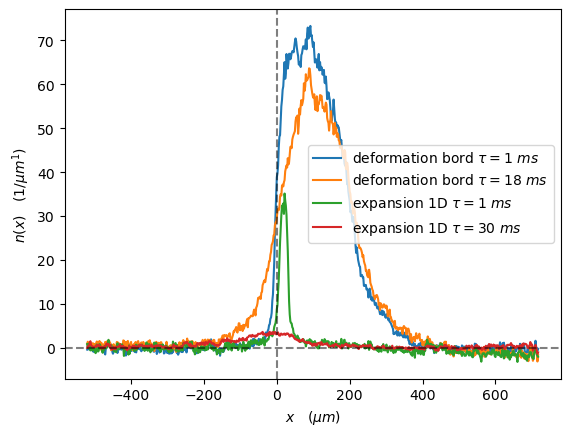
\includegraphics[width=\textwidth]{Figures/donnees_24-04-2024}
        \caption{les profiles du 24-04-2024}
        \label{fig:sub1}
    \end{subfigure}
    \hfill
     \begin{subfigure}[b]{0.45\textwidth}
        \centering
        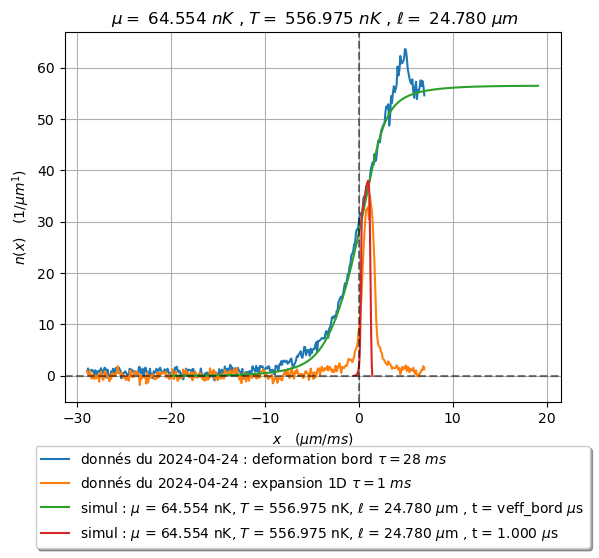
\includegraphics[width=\textwidth]{Figures/simul_deformation_18_24-04-2024}
        \caption{les profiles du 24-04-2024}
        \label{fig:sub1}
    \end{subfigure}
    
    \vspace{1em}
    \begin{subfigure}[b]{0.45\textwidth}
        \centering
        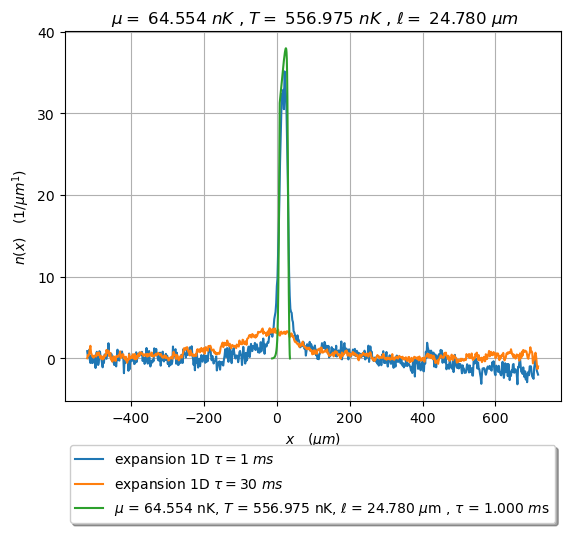
\includegraphics[width=\textwidth]{Figures/simul_expansion_1_24-04-2024}
        \caption{expansion $\tau = 1ms$}
        \label{fig:sub4}
    \end{subfigure}
    \begin{subfigure}[b]{0.45\textwidth}
        \centering
        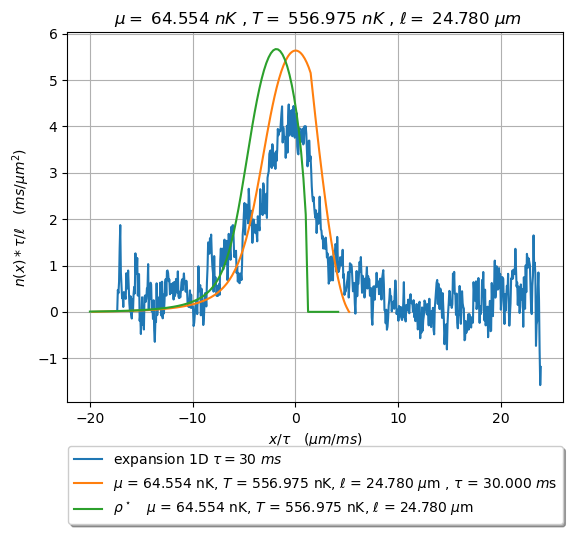
\includegraphics[width=\textwidth]{Figures/simul_expansion_30_24-04-2024}
        \caption{expensuin : $\tau = 30ms$}
        \label{fig:sub3}
    \end{subfigure}
    
    \vspace{1em}

    \begin{subfigure}[b]{0.3\textwidth}
        \centering
        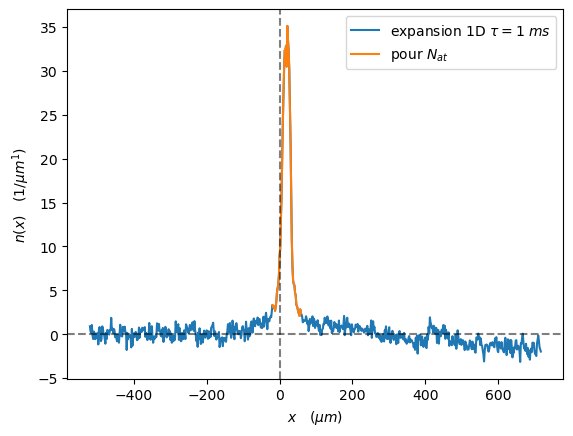
\includegraphics[width=\textwidth]{Figures/donnees_expansion_1_24-04-2024}
        \caption{expensuin : $\tau = 1ms$}
        \label{fig:sub2}
    \end{subfigure}
	\hfill
    \begin{subfigure}[b]{0.3\textwidth}
        \centering
        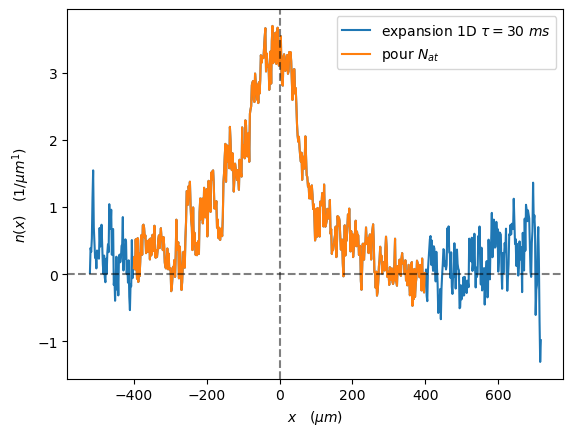
\includegraphics[width=\textwidth]{Figures/donnees_expansion_30_24-04-2024}
        \caption{expensuin : $\tau = 30ms$}
        \label{fig:sub3}
    \end{subfigure}
    \hfill
    \begin{subfigure}[b]{0.3\textwidth}
        \centering
        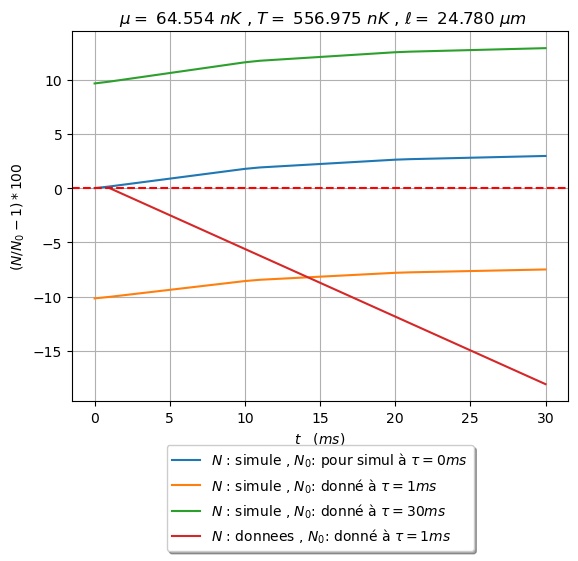
\includegraphics[width=\textwidth]{Figures/Nat}
        \caption{Nombre d'atomes}
        \label{fig:sub3}
    \end{subfigure}
    
    % Quatrième sous-figure


    \caption{Données du 24-04-2024 et simulation avec ajustement sur déformation du bord , où $\mu = f(T , n_p)$ avec $n_p$ mesuré sur donné "déformation bord $\tau = 1ms$}
    \label{fig:main}
\end{figure}

\begin{figure}[ht]
    \centering
    % Première sous-figure
    \begin{subfigure}[b]{0.45\textwidth}
        \centering
        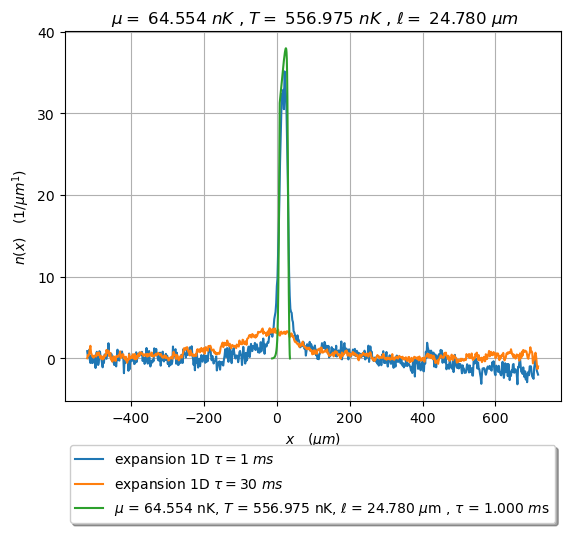
\includegraphics[width=\textwidth]{Figures/simul_expansion_1_24-04-2024}
        \caption{expension : $\tau = 1ms$}
        \label{fig:sub1}
    \end{subfigure}
    \hfill
     \begin{subfigure}[b]{0.45\textwidth}
        \centering
        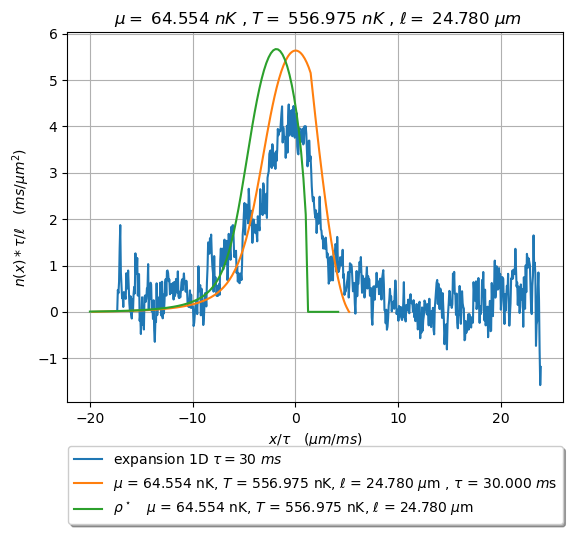
\includegraphics[width=\textwidth]{Figures/simul_expansion_30_24-04-2024}
        \caption{expension : $\tau = 30ms$}
        \label{fig:sub1}
    \end{subfigure}
    
    \vspace{1em}
    \begin{subfigure}[b]{0.45\textwidth}
        \centering
        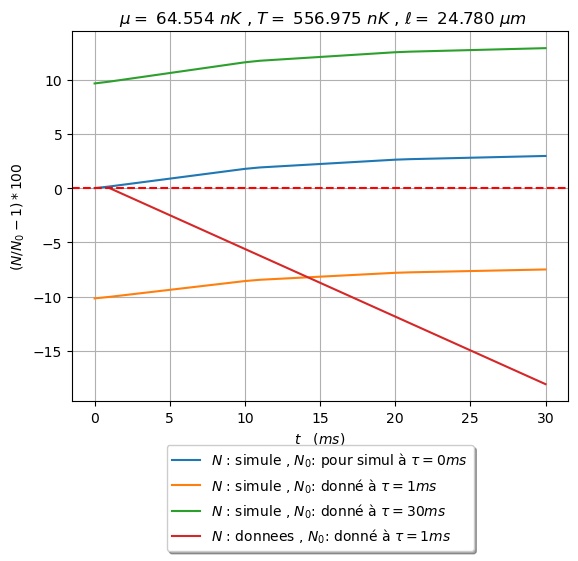
\includegraphics[width=\textwidth]{Figures/Nat}
        \caption{Nombre d'atomes}
        \label{fig:sub4}
    \end{subfigure}
    \begin{subfigure}[b]{0.45\textwidth}
        \centering
        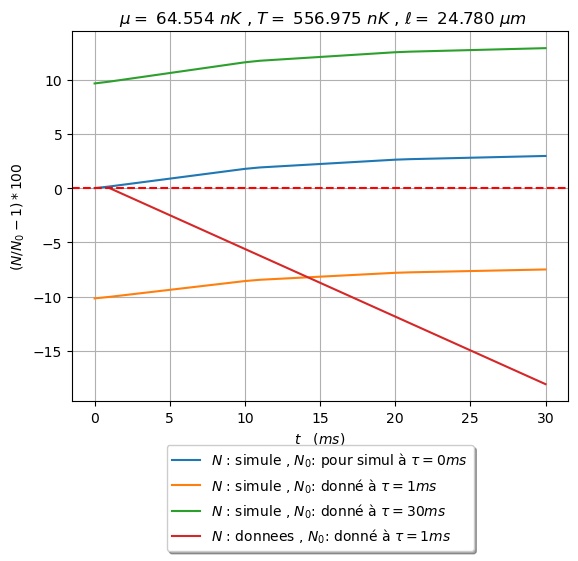
\includegraphics[width=\textwidth]{Figures/Nat}
        \caption{Nombre d'atomes}
        \label{fig:sub3}
    \end{subfigure}
    
    

    \caption{Données du 24-04-2024 et simulation avec ajustement sur expension du bord , où $\mu = f(T , n_p)$ avec $n_p$ mesuré sur donné "déformation bord $\tau = 1ms$}
    \label{fig:main}
\end{figure}
	
\end{document}


	